\chapter{Storyboard}

Nessa Storyboard é apresentada uma situação onde um estudante da Universidade de Brasília (UnB) utiliza o sistema de matrícula (Matrícula Web) da universidade e 
percebe que o sistema apresenta alguns problemas, então ele reclama sobre isso com uma colega da universidade, que o aconselha a usar o aplicativo MyPush. 
A história se passa no quarto do aluno e na UnB. 

Dados os problemas inerentes ao “Matrícula Web”, como dificuldade de acesso a oferta de disciplinas do semestre, o usuário é motivado a utilizar o aplicativo 
para obter as informações das disciplinas sem precisar acessar o sistema da universidade. Assim, para ver a oferta do semestre, bastou ele escolher as disciplinas 
que desejava cursar e o dia que desejava receber a notificação, e o aplicativo notificou a oferta no dia solicitado. 
A Storyboard pode ser vista na sua versão em papel no Apêndice e na ferramenta BitStrips na Figura ~\ref{fig:storyboard}.

\begin{figure}[!htb]
 \centering
 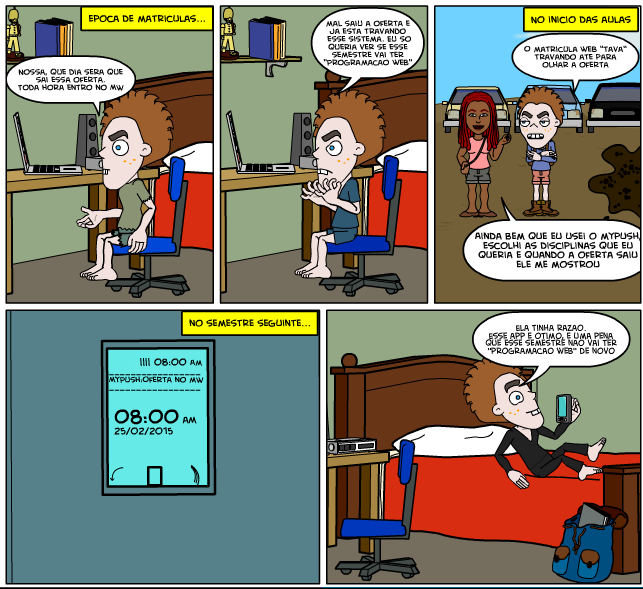
\includegraphics[width = 15.5cm, height = 13cm]{storyboard}
 \caption{Storyboard na Ferramenta}
 \label{fig:storyboard}

\end{figure}
